\documentclass[12pt,a4paper]{report}
\usepackage[spanish,mexico]{babel} 
\usepackage[utf8]{inputenc}
\usepackage{setspace}
\usepackage[top=2.4cm, bottom=2.7cm, left=3.3cm, right=2.0cm]{geometry}   % with the script is lower the text, with kile it put +o- 1 cm above, check when pinted in the school
%\usepackage[square, comma, sort&compress]{natbib}
\usepackage{makeidx}
\setcounter{secnumdepth}{3}
\setcounter{tocdepth}{3} 		
\usepackage{url}
\usepackage{subfig}  % para usar la función subfigura
\usepackage{epsfig}  % para trabajar con figs eps 
\usepackage{multirow}
\usepackage{bigstrut}
\usepackage{booktabs}
\usepackage{rotating} 				% for vertical text in tables with  \begin{sideways}Paper\end{sideways} &\begin{sideways}Static\end{sideways} \\
\usepackage{algorithm}
%\usepackage[numbered]{algo}
%\usepackage[printonlyused,withpage]{acronym}
\usepackage{hyphenat} 			%hyphenation of compound words
\usepackage{array} 			% to increse space between rows in tables using \setlength{\extrarowheight}{1.5pt}
%\usepackage{multicol}
\usepackage{pdflscape} 			% for landscape some pages
\usepackage{textcomp} 			% for the +- sign \textpm
\usepackage{acronym}
\usepackage{graphicx}

\graphicspath{ {images/} }

\makeindex

\begin{document}

    \begin{titlepage}
    \begin{center}
    \vspace*{1.0in}
    {\LARGE Aprendizaje Incremental para la Tarea de Reconocimiento de Digitos con Redes Neuronales Artificiales}
    \par
    %\vspace{0.2in}
    %{\LARGE hh}
    %\par
    \vspace{0.5in}
    {by}
    \par
    \vspace{0.2in}
    {\large Gonz\'alez Hern\'andez Luis \'Angel}
    \par					% blank line
    %\vfill 					%strech vertical space so that it fills all empty space 
    \vspace{2in}
    
    \par
    \vspace{2in}
    \begin{flushright}
     
    
    CUUAEM VM \\
    UAEM\
    Diciembre 2022
    
    \end{flushright}
    
    \end{center}
\end{titlepage}
    \pagenumbering{roman}
    \newpage
    \thispagestyle{empty}
    % Empty page


    % put double spacing
    \doublespacing

    \thispagestyle{empty}
    %1-2 pages
    \begin{abstract}

        El aprendizaje incremental es un área de la Inteligencia Artificial la cual permite agregar nuevo conocimiento 
        a un modelo (e.g. Redes Neuronales Artificiales) sin la necesidad de entrenar el modelo con toda la información 
        histórica de la tarea en cuestión \cite{bullinaria2009}. En el presente trabajo de investigación se ocupará el modelo de Redes 
        Neuronales Artificiales enfocada en la clasificación de dígitos escritos a mano usando el algoritmo de 
        entrenamiento de backpropagation, con redes Multi capa Perceptron y duplicación de pesos múltiples 
        simulando memoria a corto y largo plazo para mejorar los resultados presentados en \cite{bullinaria2009}.\\

    \end{abstract}

    \newpage
    \thispagestyle{empty}
    % Empty page

    % dedication
    \newpage
    \thispagestyle{empty}

    %  \addvspace{3in}
    \vspace*{2in}


    \noindent \hspace{2in} Dedicatoria 

    \newpage
    \thispagestyle{empty}
    % Empty page
    ~

    \chapter*{Agradecimientos}
    \thispagestyle{empty}


    Sus agradecimientos

    \tableofcontents

    \listoffigures

    \listoftables

    % \listofalgorithms


    \newpage
    \thispagestyle{empty}
    % Empty page
    ~

    % A c r o n y m s
    \chapter*{Lista de Acronimos}


%%%%%%%%%%%%%%%%%%%%%%%%%%%%%%%%%%%%%%%%%%%%%%%%%%%%%%%%%%%%%%%%%%%%%%%%%%%%%%%%%%%%%%%%%%%%%%%%%%%%%%%%%%%%%%%%%%%%%%%%%%%%%%%%%
% Rules for this pacage
% \ac{ acronym } 	put it, put full acronym if it is the first time
% \acresetall 		flushed the memory of macro \ac, so it will print the full acroym the first time any of them is called
% \acf{} 		Full name is printed, and the acronym is in brackets
% \acs{}		short version
% \acl{} 		expanded acronym without even mentioning the acronym

% \acp			Works in the same way as \ac, but makes the short and/or long forms into plurals.
% \acfp			Works in the same way as \acf, but makes the short and long forms into plurals.
% \acsp			Works in the same way as \acs, but makes the short form into a plural.
% \aclp			Works in the same way as \acl, but makes the long form into a plural.
% \acfi			Prints the Full Name acronym (\acl) in italics and the abbreviated form (\acs) in upshaped form.
% \acused		Marks an acronym as used, as if it had been called with \ac, but without
% 			printing anything. This means that in the future only the short form of the
% 			acronym will be printed.
% 
% \acsu			Prints the short form of the acronym and marks it as used.
% \aclu			Prints the long form of the acronym and marks it as used. Example: \acl{lox}/\acl{lh2} (\acsu{lox}/\acsu{lh2})
% \...*			The following commands do the same as their unstarred forms, except that the
% 			acronym will not be marked as used. If you work with the ’onlyused’ option then
% 			macros which have only been used with starred commands will not show up.
% 			\ac*, \acs*, \acl*, \acf*, \acp*, \acsp*, \aclp*, \acfp*, \acfi*, \acsu* and
% 			\aclu*.
%
% For more information see the manual: /media/dat/LIBROS/Latex/acronyms/acronym.pdf
%%%%%%%%%%%%%%%%%%%%%%%%%%%%%%%%%%%%%%%%%%%%%%%%%%%%%%%%%%%%%%%%%%%%%%%%%%%%%%%%%%%%%%%%%%%%%%%%%%%%%%%%%%%%%%%%%%%%%%%%%%%%%%%%%




% Previous version

%\begin{table}[b]
  	%\caption{Multiple-step, closed-loop or iterate forecasting}
%		\centering
%			\begin{tabular}{llll}
				%\hline\noalign{\smallskip}
				%${Forecast}$ & $Inputs$ \\
				%\noalign{\smallskip}
				%\hline
				%\noalign{\smallskip}
%& MSP & & Multi step prediction \\
%& SSP & & Single step prediciton \\ 
				
				%\hline
%			\end{tabular}\\
%			\vspace{-2mm}
%		\label{MultipleForecasting}
%	\end{table}

    %\newpage

    \pagenumbering{arabic}

    % put double spacing
    \doublespacing



    % Each one is a chapter 
    \section{Introduccion}

El aprendizaje incremental es un método el cual a sido implementado en el área de la inteligencia artificial, ya que al realizar tareas especificas de dicha rama nos 
ayuda a optimizarla para que el algoritmo sea más eficiente.
Cualquier tipo de aprendizaje puede ser considerado aprendizaje incremental si el problema a resolver tiene un entrenamiento simple, adem\'as este tipo de algoritmo es conocido como \textit{algoritmo lineal sin memoria},
en la mayor\'ia de los casos este tipo de aprendizaje es el preferido o favorito por los desarrolladores \cite{GiraudCarrier2000}.

Las redes neuronales artificiales (RNAs) son procesos matem\'aticos los cuales son utilizados en el \'area de Machine Learning para 
la resoluci\'on de problemas no lineales, estos deben de pasar por una funci\'on de activaci\'on la cual es una multiplicaci\'on 
entre lo valores otrogados, al ser procesados por las capas que contenga la neurona, obtendremos un valor distinto al de entrada.

Adem\'as son una distribuci\'on muy conocida de parte del Machine Learning, de otra manera es el poder que tienen las computadoras para una buena estructura distribuida en paralelo y una buena habilidad de aprendizaje, 
este modelo computacional se define por medio de las neuronas biologicas las que son encargadas de que el ser humano pueda aprender o distinguir de distintos aspectos, este tipo de 
metodo es motivado para poder obtener la meta de un buen aprendizaje de maquina \cite{liu2015}.

Un factor importante para esta rama es la perdida de memoria, este es un problema biol\'ogico, el cual tanto afecta a los humanos como a las maquinas, es por eso que se han elaborado distintos
experimentos para poder convatir esta problematica.
Uno de  estos es el caso de John Bullinaria, quien maneja la arquitectura de doble peso, ya que en su experimento da a notar que mejora la utilizaci\'on del aprendizaje incremental, esto se logro 
con sistemas existentes como lo es Learn++.

Cabe mencionar que el experimento realizado fue un problema de generalizaci\'on m\'as comunes, pero se necesitan m\'as evidencias 
de que usando esta metodolog\'ia sirve para utilizarlo no solamente en tareas generalizadas, adem\'as se espera un mejor rendimiento \cite{Bullinaria2009}.  \\


\section{Planeamiento}

    Indicar de forma general como es el funcionamiento de las redes neuronales en el uso general, como es que se produce la falta de memoria en 
    estos modelos de predicciones. Poner en pr\'actica los modelos de experimentación de John Bullinaria para comprobarlos con
    problematicas m\'as robustas y optimizarlo para que sea un m\'etodo eficiente.

    \newpage
    \thispagestyle{empty}
    % Empty page
    
    \chapter{Revisión de la Literatura}
  \section{Redes Neuronales Artificiales}
  
    Las redes neuronales artificiales (RNA) son modelos computacionales de la Inteligencia Artificial los cuales contienen simples unidades de procesamientos llamadas neuronas.  Ellas se inspiran en el cerebro humano, tomando como base la conectividad entre neuronas y el aprendizaje que pueden tener.  Un perceptron o neurona (artificial) solamente resuelve problemas lineales y tiene la siguiente forma:
    
    \begin{figure}[H]
      \centering
      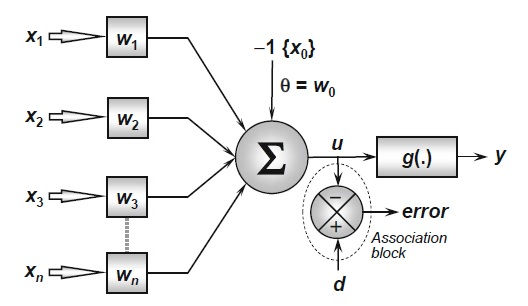
\includegraphics[width=\columnwidth]{ANN.jpg}
      \caption{Red Neuronal Artificial B\'asica}
      \label{fig:fig1}
    \end{figure}

    Donde $\Sigma$ es la representación matemática de la neurona.,  $x_1$, $x_2$,  \dots  ,$x_n$ son las variables de entrada a la red.  $w_1$,$w_2$,  \dots , $w_n$ son los pesos con los cuales se van a podnerar las entradas, es decir multiplicar cuando la información entra en la neurona. Posterior a multiplicar el peso por la entrada correspondiente,  se suman todos esos valores $w_1$$x_1$ + $w_2$$x_2$ + $w_3$$x_3$.


    \section{Metodología}
    El primer paso a realizar en esta investigación es recrear el código mostrado en \cite{bullinaria2009}, donde se describe la implementación de una red  neuronal multicapa usando el algoritmo de entrenamiento backpropagation en el lenguaje de programación Python.  Para esto se utilizará el conjunto de datos de Optical Digits,  en donde se tendrá que preprocesar los datos, para eliminar registros inválidos. 

    Posteriormente se implementará una nueva versión del código en donde se experimentará con mas de dos capas de pesos duplicados para mejorar la tasa de olvido de información al momento de usar el aprendizaje incremental.  Para ello se explorará incrementando gradualmente el nueron de capas (esto no lo entendi,neuronas de capas?)de pesos duplicados, hasta llegar al punto en que mas capas no generen un decremento de las tasas de olvido/error.

(REVISEN LA REDACCIÓN Y MEJORENLA DE FAVOR)
    Cuando los dos proyectos se tengan, se realizar\'a una comparación, donde se ver\'a cual de estos dos experimentos
    es más eficaz en proyectos de la vida real.
    
\section{Cronograma de Actividades}
(EL CRONOGRAMA DE ACTIVIDADES DICE JOHN BULLINARIA EN LA PARTE DE ARRIBA, ELIMINAR ESO)

    \begin{figure}[H]
        \centering
        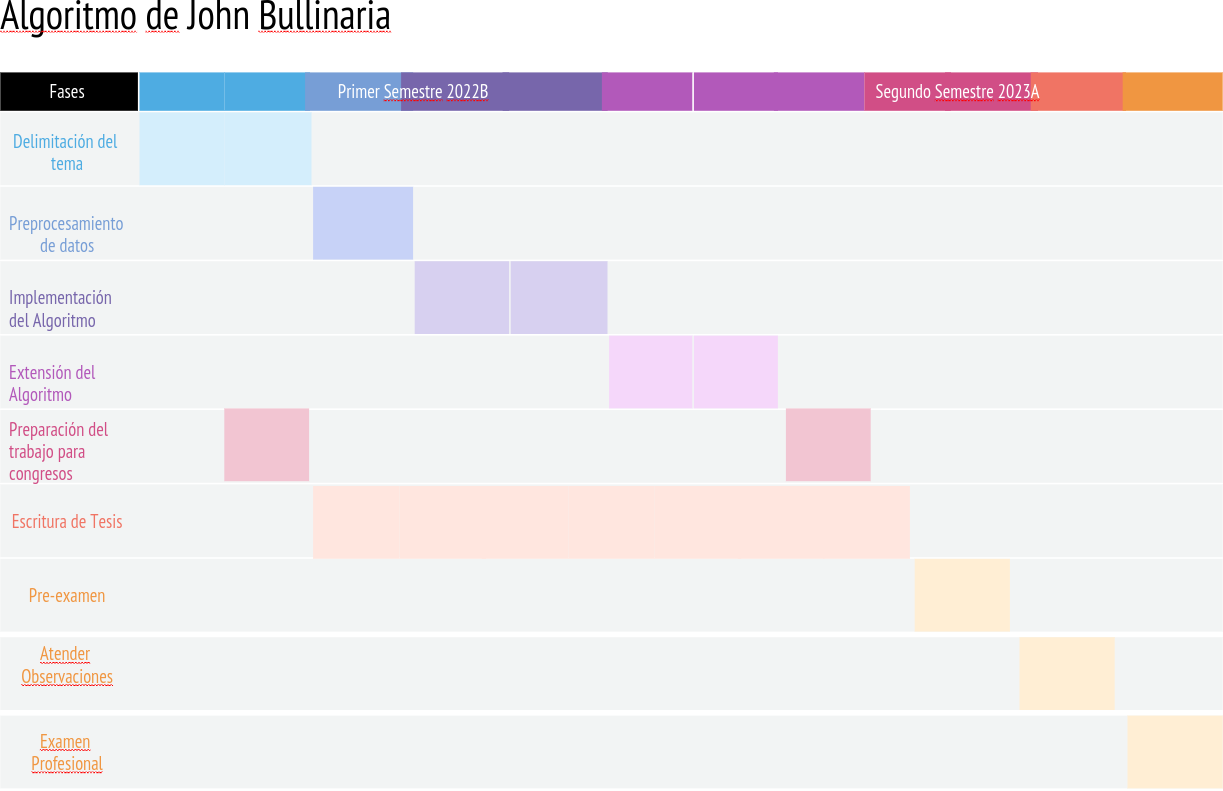
\includegraphics[width=\columnwidth]{diagramaGantt.png}
        %\caption{Elimine estoa horita, no hace falta ponerle un titulo, dado que es la únic figura en la sección}
        \label{fig:fig3}
    \end{figure}

\section{Organización del Capitulado}


	En el capitulo 2 se ver\'a lo que es el aprendizaje humano y el aprendizaje incremental con sus algoritmos, se describirán las redes neuronales artificiales.

En el capitulo 3 se implementar\'a el articulo de John A. Bullinaria, como funciona, resultado que da al pasar los datos que dice para comprobar que funciona como menciona en su art\'iculo. En el capitulo 4 se explicar\'a como se hará la modificación a su algoritmo, cuantas capas se van a poner, como se van a repartir las tazas de aprendizaje.

Posteriormente en el capitulo 5 se mostrar\'a una comparación de los resultados de ambos trabajos. En el capitulo 6 se verán las conclusiones y trabajo futuro.



    %\bibliographystyle{acm}
    \bibliographystyle{ieeetr}%plain}
    \bibliography{dataset.bib}
    %\bibliography{BaseDatos2}


%\printindex
\end{document}

